% !TEX options=--shell-escape
\documentclass[12pt]{article}
\usepackage{graphicx}
\usepackage{float}
\usepackage{minted}
\usepackage{listings}
 \usepackage{color} 
 \usepackage{mdframed}
 %\usepackage{courier}
\definecolor{mygrey}{gray}{0.95} % Light Gray

% Title.
\title{Experiment 2\\ Eight-Bit ALU Design}
% Author
\author{Amit Kumar,16D070034}

% begin the document.
\begin{document}

% make a title page.
\maketitle

% section 1: overview.
\section{Overview of the experiment}

ALU (Arithmetic Logic Unit) is a importaant unit which can perform simple arithmetic and logical operations. In this experiment I have designed a 8-bit ALU which performs the following task :\\
\begin{itemize}
\item Addition
\item Substraction
\item Logical Right-Shift
\item Logical Left-Shift
\end{itemize}
The code was compiled on ALTERA Quartus Prime, and simulated using ModelSim which was then uploaded to the Krypton v1.1 \textit{5M1270ZT144C5N} CPLD-based board.

% The codes and setup have been covered in section 1. We build the ALU piece-wise, by imple-
% menting each module independently. The VHDL codes have been kept modular and as generic

% as possible, for reusability and code clarity. Section 2 presents the simulation observations and
% miscellaneous results.

\section{Experiment setup \& approach}

%Describe the experimental setup (or the approach you have used
%to complete the assignment).
We implemented the above operations step by step starting from basic logic gates which is mentioned in particular sections later.

We have to do these operations on two eight numbers. So there are two 8-bit inputs X and Y, and it produces an 8-bit output Z. The operation to be
performed is selected by a 2-bit operation code (opcode). The functionality
of the ALU based on the op code bits is shown in Table 1.

\begin{table}[H]
\centering
\begin{tabular}{| c | c | c |}
\hline
Op Code(opcode) & Operation & result \\
\hline
00 & Addition & Z = X + Y \\
01 & Substraction & Z = X - Y \\
10 & Logical Right-Shift & Z = X $>>$ Y \\
11 & Logical Left-Shift & Z = X $<<$ Y \\
\hline
\end{tabular}
\caption{Op-codes for the ALU}
\end{table}


\subsection{Addition}
For Addition, I designed \textbf{half adder} which takes two bits as input and gives their sum bit and carry bit .\\  Logic :\\ $ s_o = a \oplus b  , c_o = a.b $ \\ \\ 
\textbf{Half Adder}
\inputminted[fontsize=\footnotesize,linenos,frame=lines
]{VHDL}{HalfBitAdder.vhd}

\newpage
 I used two half adders to make a \textbf{full adder} which takes three inputs ( two bits to be added and a carry$_{in}$ bit and gives their sum and carry bit.\\ Logic : \\ $$s_o = a \oplus b \oplus c_{in} , c_o = ab + bc_{in} + ac_{in}$$
 \\ \textbf{Full Adder} 
 \\  \\
%\lstinputlisting{mux.vhd}
\inputminted[
% frame=lines,
 %framesep=2mm,
%baselinestretch=1.2,
bgcolor=mygrey,
fontsize=\footnotesize,
linenos
]{VHDL}{FullBitAdder.vhd}
\\ \\
Finally I used a series of full adders to implement add eight bits and outputs their sum.
\\ \\
 \textbf{Eight Bit Adder} 
\inputminted[
% frame=lines,
 %framesep=2mm,
%baselinestretch=1.2,
fontsize=\footnotesize,linenos,frame=lines
]{VHDL}{EightBitAdder.vhd}
\subsection{Substractor}
For the Substractor, I have used the 2's complement approach which is done by using the previous eight bit adder with an additional bit '1' to cin of the first full adder. \\
Let a' be 2's complement of a, so\\ 
 $ b + a' = b + ( 2^n - 1 - a ) = (b - a) + 2^n -1 $ \\ Here additional one is added to care of 
 $-1$ and $2^n$ is taken into account by taking n-bits only as it will appear at (n+1)th bit.\\
 \\ \textbf{Substractor}
\inputminted[fontsize=\footnotesize,linenos,frame=lines
]{VHDL}{Substractor.vhd}

\subsection{Logical Right Shift}
% The logical right shift is an essential operation for an ALU. One of the simplest interpretation
% can be division by 2. This can give an easy way to implement multiplication/division operations.
% Hardwiring is always an option, but a more general and reusable algorithm would be preferred.
For this part, I perform shifts using logarithmic barrel shifting. An illustration of barrel-shifting is given in figure 1. Note that although both X, Y are 8-bit, if Y is more than 111, then the output would be monotonously zero. So, we need to implement only 3 stages.\\
\begin{figure}[H]
\begin{center}
\includegraphics[width=14cm]{Rshift.png}
\caption{Logarithmic barrel shifter Logic for Right Shifter}
\end{center}
\end{figure}
So, I created a mux entity, which is then used to make the 8-mux chains, eventually making our shifter.\\logic : \\ $$o = a*\bar{s} + b*s $$ \\
\textbf{MUX}
\inputminted[fontsize=\footnotesize,linenos,frame=lines
]{VHDL}{mux.vhd}

\noindent Then I implented 8-mux chains to shift 1 bit, 2 bits and  bits respectively.\\ \\ \\
\textbf{MUX chain for 1-bit shifting } 
\inputminted[fontsize=\footnotesize,linenos,frame=lines
]{VHDL}{mux_chain_1bit.vhd}
\noindent Implementation of mux chain for 2 bit shift\\ \\
\textbf{MUX chain for 2-bit shifting } 
\inputminted[fontsize=\footnotesize,linenos,frame=lines
]{VHDL}{mux_chain_2bit.vhd}

\noindent Implementation of mux chain for 4 bit shift\\ \\
\textbf{MUX chain for 4-bit shifting } 
\inputminted[fontsize=\footnotesize,linenos,frame=lines
]{VHDL}{mux_chain_4bit.vhd}

\noindent Implementation of an additional mux chain to convert the output to zero when number to shift is greater than three bits.\\ \\
\textbf{MUX chain for implementation with 8 bit input } 
\inputminted[fontsize=\footnotesize,linenos,frame=lines
]{VHDL}{mux_ALU.vhd}

\noindent Implementation of an additional mux chain to reverse the bits from LSB side to MSB side for implentation of both Lshift and Rshift with same logic.\\ \\
\textbf{MUX chain for reversing bits } 
\inputminted[fontsize=\footnotesize,linenos,frame=lines
]{VHDL}{mux_change.vhd}

\noindent Final implementation of Right shifter using above components.\\ \\
\textbf{Right Shifter } 
\inputminted[fontsize=\footnotesize,linenos,frame=lines
]{VHDL}{Rshift.vhd}

\subsection{Logical Left Shift}
It is implemented with same logic as right shift. Just I havereversed the incoming bits and the respective output .
\\ \\
\textbf{Left Shifter } 
\inputminted[fontsize=\footnotesize,linenos,frame=lines
]{VHDL}{Lshift.vhd}

\section {ALU}
Integrating all the above components and testbench used are given below.\\
\\
\textbf{ALU } 
\inputminted[fontsize=\footnotesize,linenos,frame=lines
]{VHDL}{alu.vhd}
\noindent Implementation of final DUT to be tested by testbench \\ 
\\  \noindent \textbf{DUT } 
\inputminted[fontsize=\footnotesize,linenos,frame=lines
]{VHDL}{DUT.vhd}

\\  \noindent \textbf{Testbench } 
\inputminted[fontsize=\footnotesize,linenos,frame=lines
]{VHDL}{Testbench.vhd}


\section{Observations}
All te relevant screenshota and results are shown below:\\
\begin{figure}[H]
\begin{center}
\includegraphics[width=16cm]{transcript_gatelevel.png}
\caption{Transcript window of all test case passed with GATE level simulation}
\end{center}
\end{figure}
 
 \begin{figure}[H]
\begin{center}
\includegraphics[width=20cm]{gat_initi_error.png}
\caption{Initial waveforms obtained from gate level simulation}
\end{center}
\end{figure}
 
  \begin{figure}[H]
\begin{center}
\includegraphics[width=20cm]{gate.png}
\caption{Comparison of output obtained by testbench and tracefiles for ALU}
\end{center}
\end{figure}
 
 \begin{figure}[H]
\begin{center}
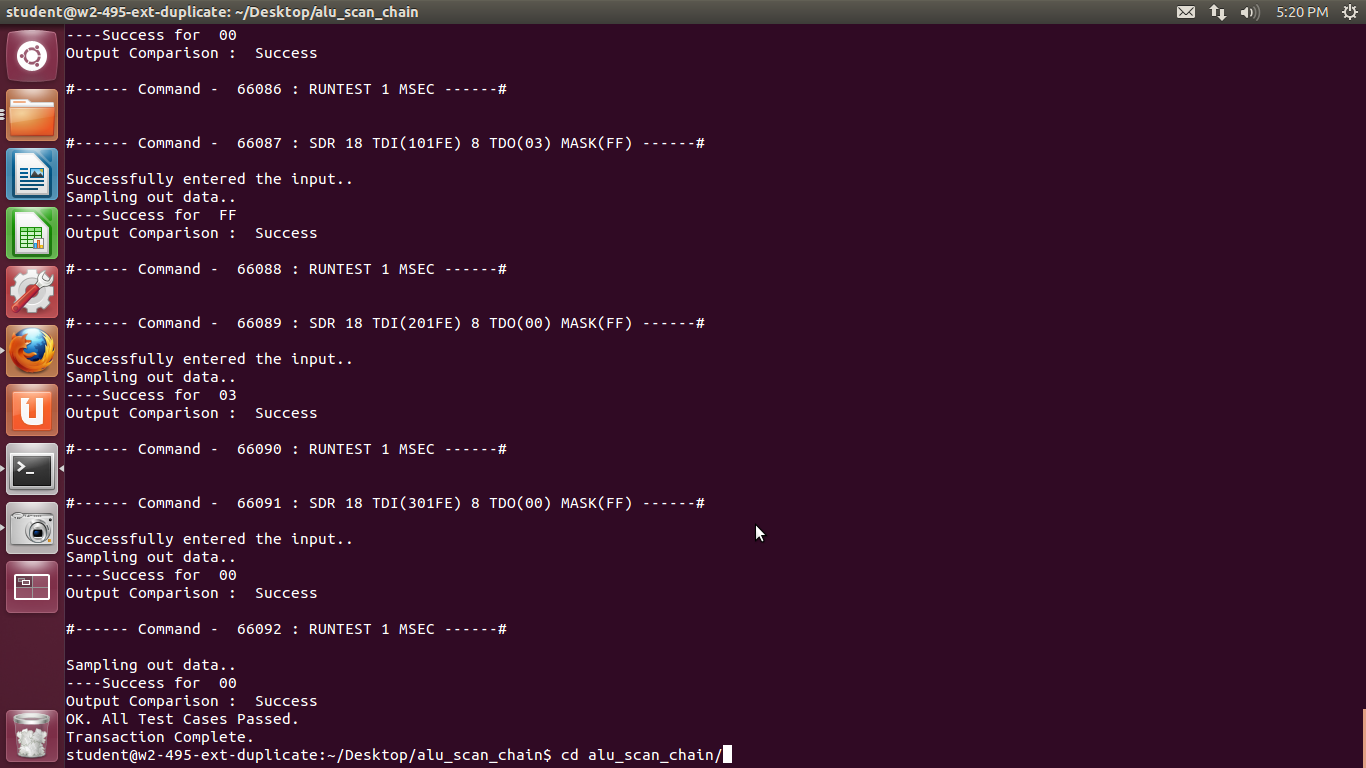
\includegraphics[width=20cm]{scp.png}
\caption{Screenshot of all test case passed using Scan chain}
\end{center}
\end{figure} 

 \begin{figure}[H]
\begin{center}
\includegraphics[width=20cm]{schain.png}
\caption{Output file obtained by scan chain}
\end{center}
\end{figure} 

\end{document}
